\section{Blockchain Limitations and Proposed Approach}
\label{sec:limitations}

\footnote{This section was contributed by Martin Uzak, Aptoide's backend team member}
The current status of blockchain developments, both Bitcoin and Ethereum, can limit the development of projects that depend on the technology to support the required business use cases. %missing citation?
 
There are three use cases which the AppCoin protocol tries to solve in order to enable a fully working AppCoin economy:

% \subsection{Use Cases}

\begin{itemize}
    \item Apps advertising in app store
    \item In-App Billing 
    \item Developer reputation leading to apps approval
\end{itemize}

From the above-mentioned use cases a list of requirements on the technology can be established. 

\begin{itemize}
    \item Store digital value securely
    \item Couple value storage and transfers with logic
    \item Scalability for millions of users
\end{itemize}

The first requirement is solved by using a blockchain technology. Both Bitcoin or Ethereum work for this. For the second requirement only a blockchain technology supporting smart contracts will work, i.e. Ethereum, Nxt or Tezos.

Unfortunately, bare Ethereum nor any other current blockchain for that matter are able to scale for the needs of an app marketplace. This problem is even more aggravated considering a platform potentially working for all the app marketplaces.

First let us have a detailed look at the challenges in question.

\subsection{Blockchain limits}


Let's try to imagine a scenario of a working AppCoins economy using a bare blockchain technology like Ethereum.

At the present there are about 2 billion Android users. The average Ethereum transaction is around 160 bytes \cite{EthereumTransactions}. If we wanted to create an AppCoin economy directly on Ethereum using these numbers, we would get a system with the characteristics shown in Table \ref{table:ethereumscalability}.

\begin{table}[!htbp]
\centering
\begin{tabular}{|l|r|}
\hline
Users              & 2 000 000 000    \\ \hline
Avg. daily TX      & 1                \\ \hline
Avg. TX size       & 160 bytes        \\ \hline
Daily TX           & 2 000 000 000    \\ \hline
TX per second      & 23 148           \\ \hline
Daily TX size      & 298.02 GB        \\ \hline
TX size per second & 3.53 MB          \\ \hline
TX size per month  & 8.73 TB          \\ \hline
TX size per year   & 104.77 TB        \\ \hline
\end{tabular}
\caption{Scalability requirements for AppCoin economy}
\label{table:ethereumscalability}
\end{table}

\medskip

{\bf Transaction Volume}

Scalability in terms of volume is the first problem of Ethereum. At the present it handles only up to 20 transactions per second \cite{eth_scaling}. That is nowhere near the required 23 000 average transactions per second. For peak times the system should support a number of transactions several orders of magnitudes higher. E.g., VISA handles normally around 1667 and at peak times it claims it can do around 56 000 per second \cite{eth_scaling}.

\medskip

{\bf Fees}

The topic of fees is closely connected to the possibility to support micro transactions - transfers of value in the range of a few cents. At the time of writing the cost for one transaction in Ethereum is around 10 cents of a US Dollar for a transaction that takes around 1 minute to execute \cite{ethgasstation}. If the user is willing to wait around 10 minutes, the cost is 1 cent. This is both too slow and too expensive to facilitate micro transactions.

\medskip

{\bf Latency}

As mentioned in the previous section, in Ethereum, one has to wait until a transaction is part of the blockchain. To have a reasonable guarantee that the transaction is part of the main blockchain and not of one of possible branches, one needs to wait 7 blocks. This is because two miners could submit the next block at the same time and it will take some time to decide whose block will continue the chain. While this might not be an issue for high value money transfers in the AppCoin economy the transactions have to be executed within few seconds or faster (preferably instantly) in order to enable meaningful IAB and user experience.

\subsection{Existing technology}

Scalability restrictions are present in any blockchain technology using mining by \textit{proof-of-work} e.g. Bitcoin and Ethereum. For Bitcoin - the oldest blockchain implementation - the proposed solution is the Lightning Network \cite{LighthingNetwork}.

%why is the lightning network the only solution referred? should talk about proof-of-stake?

\subsection{Ethereum and Bitcoin based}

Basically there is one possibility how to tackle the scalability problem with Bitcoin and two solutions with Ethereum. The first one is keeping the proof-of-work based blockchain and enhancing it with a direct-channel-payment solution like the Lightning Network. For Ethereum there are two major technologies that are going to be introduced also in this section.

\subsection{Lightning Network}
In brief the Lightning Network allows for creation of bidirectional payment channels that are off-chain \cite{LighthingNetwork}. Using such a channel two parties agree to deposit money into a common entity called channel and this information is stored on the blockchain. There is a 2-signature entry for the channel with the total sum of the deposit saved. From this moment on the two parties can exchange between them any number of payments in the form of signed receipts. The only condition is that the balance for one party doesn't exceed the total of the deposit. Should a case like this happen, the parties can increase the deposit. These off-chain transactions are signed and sent direct. They are not broadcast. In contrast all the transactions on the main blockchain need to be broadcast to all participants. 

This approach solves the blockchain scalability problem, such as:

\begin{itemize}
    \item The messages are direct and not broadcast. The volume of transactions between the two parties is only limited by their processing capabilities. Also compared to blockchain not all the transactions have to be stored but only the latest receipts, i.e. the latest balance for both users. This solves the problem of storing huge amounts of old transactional data that is inherent in blockchain.
    \item The only fees are for opening and closing the payment channel on the blockchain. For payments over the payment channel there are no extra fees. Once it is established micro transactions are possible without further limitations.
    \item Finally by using direct peer-2-peer communication, transactions can be exchanged as fast as the underlying network between the two parties will enable it. Thus the problem of latency is solved.
\end{itemize}

Thus the original blockchain scalability limitations are resolved for the case of two directly connected parties. Of course having open channels between all the participants in the AppCoin economy is both not feasible and economically viable (because of opening and settling fees on the blockchain). Therefore the Lightning Network proposes a solution, where the payment channels are stored in a graph and payment can be routed securely keeping the above mentioned characteristics among multiple parties. This is enabled using hashlocks. For more detailed information, please have a look at either the specification of Lightning Network or the excellent introductory article \cite{starkness}.



\subsubsection{Raiden}
Raiden network is an early implementation of the Lightning Network protocol for Ethereum. Therefore, it is an off-chain scaling solution for Ethereum. It promises near-instant, low-fee and scalable payments and enables micro transactions \cite{Raiden}. Raiden runs as a network of nodes establishing payment channels among users. It uses locked funds in a smart contract in Ethereum and payments happen inside of Raiden until one party chooses to settle. Raiden will work for any Ethereum tokens implementing the ERC20 standard.

One of the key characteristics of Raiden is its maturity. Currently it is the only known technology for Ethereum with existing implementation (i.e. beyond white paper stage) enabling a working App Coin economy. It has been under development for the past two years and it is reaching a Minimal Viable Product stage, currently being in a developer preview stage.

Privacy is another key characteristic of Raiden.  All the transactions are known only to the involved parties and not public knowledge like in Ethereum.

Finally the maturity can also be seen as a weak point for Raiden. Even though it is beyond proof-of-concept stage it is not recommended to be used on the live Ethereum network by its creators.

\subsubsection{Plasma}
Plasma is defined as "scalable autonomous smart contracts" \cite{Plasma} and it is another attempt to bring the Lightning Network technology from Bitcoin to the Ethereum world. This is envisioned by means of a tree of hierarchical chains where most of the transactions can be settled in the sub-chains and do not need to go to the expensive and slow main chain. The main chain will be needed only to settle disputes coming from sub chains and would serve as final validation.

A strong point for Plasma is that it is backed by key people from both Ethereum and Lightning Network, i.e. Vitalik Buterin and Joseph Poon. Another aspect supporting Plasma it that is has been endorsed by OmiseGO to be used for their decentralised exchange and payment platform\cite{omisego_plasma}.

What speaks against Plasma at this time is the fact that the project has only a white paper, without any working code base yet.

\subsubsection{OmiseGO}
OmiseGO is an Asian payment gateway. It plans to use Ethereum and Plasma as a foundation for creating a decentralised exchange and payment platform \cite{OMG} and intends to launch their own blockchain called OMG that will be complementary to Ethereum. Ether will be then used as a medium of interchange for various asset being exchanged on their blockchain.

Here are some of the strong points of OmiseGO:
\begin{itemize}
    \item Consensus rules for high performance activity;
    \item Rapid execution and clearing. Proof-of-Stake;
    \item Handle extremely high volumes of transactions and of final delivery on Ethereum;
    \item Availability as white label e-Wallet solution
\end{itemize}

The weak points include:

\begin{itemize}
    \item The project is in a very early stage. It has been announced in the beginning of August 2017. Currently, there is only a white paper available.
    \item As a result of coupling with Ethereum the white paper recommends to validate transactions simultaneously on the Ethereum blockchain for maximum security.
\end{itemize}

%XXX leave this subsection out?

\subsection{Independent blockchains}
The second solution to achieve global consensus (blockchain) with some scalability is the use of a proof-of-work as block minting algorithm. For Ethereum this would be the Casper protocol which has been talked about a lot in the past years in the Ethereum community but which is not implemented yet. As Casper is not in use yet we will examine here other projects that have implemented minting instead of mining blocks.

A brief look will be also thrown at IOTA that solves the scalability problem by using not a blockchain, but a directed acyclic graph called Tangle.

\subsubsection{Nxt}
One of solutions not based upon Ethereum is Nxt. It is described as "an open source cryptocurrency and payment network launched in November 2013 by anonymous software developer BCNext" \cite{Nxt}. Compared to Ethereum one can see Nxt as a monolith trying to include major features from all coins. It describes itself as an modern economic system based on cryptography and blockchain technology. On the other hand Ethereum built a low platform and programming language in which one can program generic contracts.

Other major differentiation of Nxt to Ethereum is the fact that it is based on proof-of-stake for creating new blocks.

Nxt is unsuitable for creating an App Coin Economy as it targets a different scenario. Focusing on managing your business, assets and customers and interaction between them in a secure way. Not as a blockchain backed technology enabling to create generic decentralised Apps.

Another point speaking against Nxt is the fact that its beginning was obscure. 73 anonymous accounts received stakes in exchange for bitcoin accounts and it is these people who can mint new blocks. And also that there has not been much buzz around and development for Nxt recently.

\subsubsection{Tezos}
Compared to Nxt the next examined project has received a lot of attention recently and finished its ICO by raising more than \$200 million.

Tezos describes its ultimate aim to create blockchain technology working better than both Ethereum and Bitcoin. It wants to provide users with financial incentives for maintaining on-chain consensus mechanism. The main differences to Ethereum are:

\begin{itemize}
    \item Built-in consensus mechanism for governance.
    \item Decoupled from Ethereum. Separate blockchain with proof-of-stake consensus for block minting.
    \item OCaml as programming language for creating smart contracts.
    \item Design-wise Ethereum is a generic and low-level solution while Tezos aims to provide a fat protocol with a lot of features \cite{TezosEth}, not unlike Nxt.
\end{itemize}

\subsubsection{IOTA}
The goal of IOTA is to create a lightweight network that allows a machine economy. A machine economy is a situation where many IoT devices communicate and execute payments between each other. IOTA does not use blockchain but a directed acyclic graph called Tangle. Currently it is in Beta stage with a reference implementation. One of the major advertised features is that there are no fees. In Tangle each new transactions confirms at least 2 previous transactions. That is the "fee" to participate. This might delay the transaction, especially if the network is small. There are no miners. The IOTA white paper states it is quantum proof. It has got a lot of supply and the tokens are not divisible, unlike bitcoins or ethers. For a primer on IOTA see \cite{IOTA}.

\subsection{Proposed Approach}


\begin{figure}[!ht]
\centering
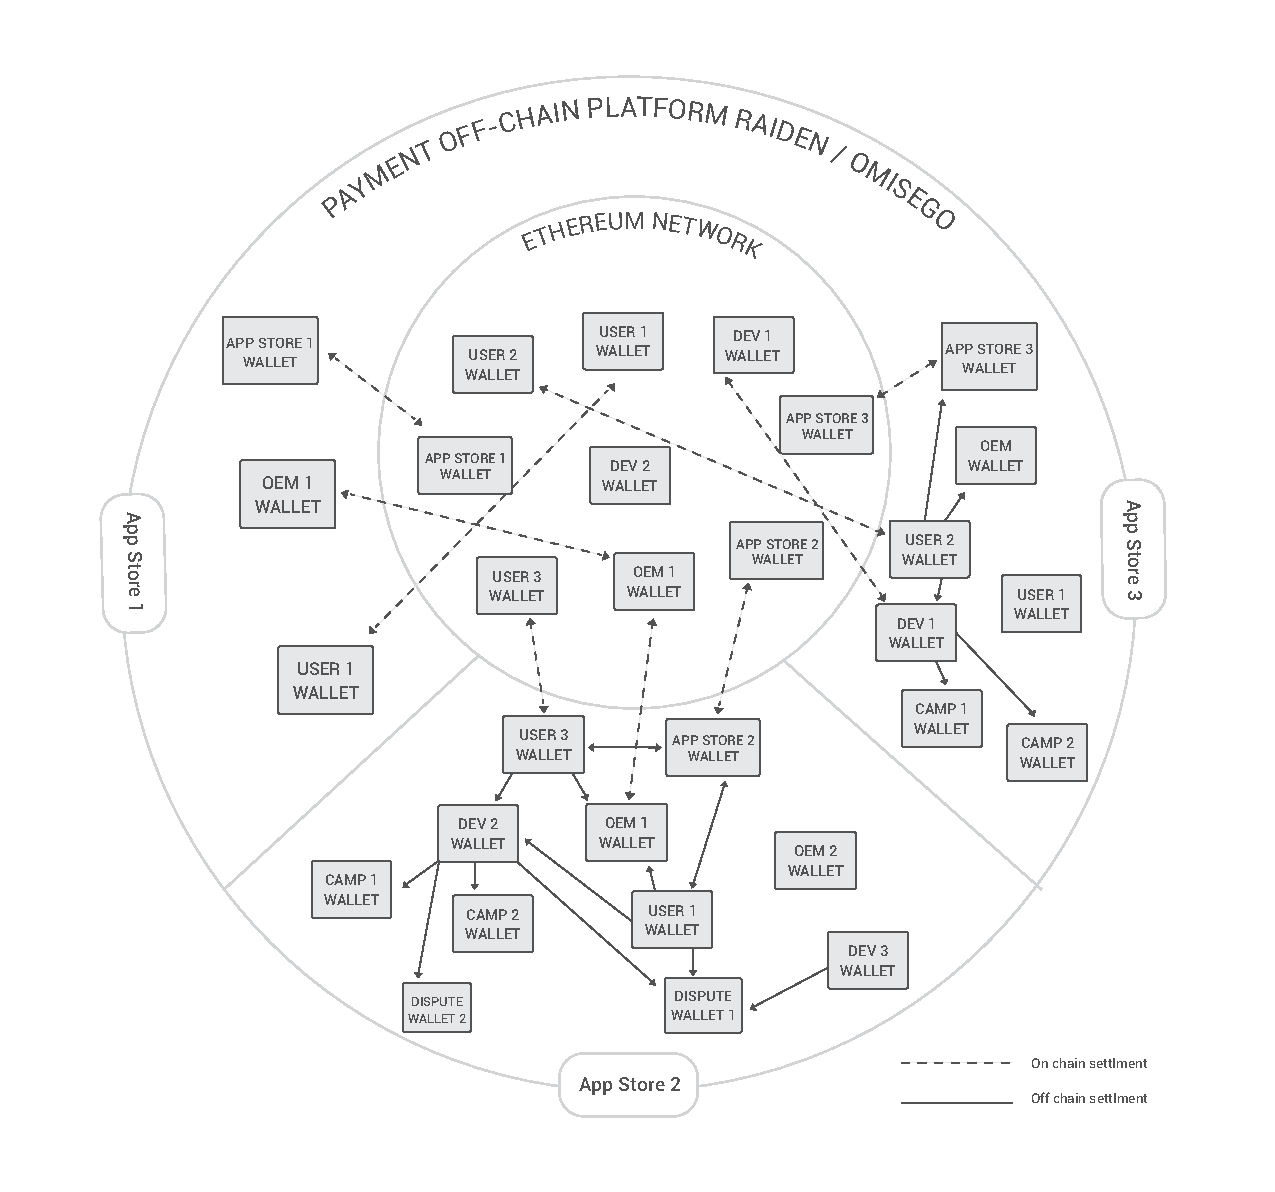
\includegraphics[width=\textwidth]{diagrams/offchain_wallets.eps}
\caption{On-chain and off-chain transactions.}
\label{fig:offchain}
\end{figure}


As seen in the previous section, there are blockchain currencies that can securely store digital value. But as we have seen, doing transactions over them does not scale, is slow and requires fees. Therefore alternatives like direct payment channels have to be evaluated.

In general terms, the App Store acts as the gateway to the digital payment world for the user. He deposits his valuables (preferably Ether) with the store in a payment channel using a smart contract. The same happens for developers. And from this moment on they can utilise the micro-payments within the App Infrastructure. The payments are instant, cheap and there can be any number of them.

The user has to pay fees on each Ether deposit to his account with the App Store and on checking out i.e. settling his payment channel. Further fees may be the taxation done by the App Store used to pay for its infrastructure.  If there are several App Stores in the same ecosystem like we envision, there might be further (minimal) fees to forward the payments from one to another.

Figure \ref{fig:offchain} depicts what is on-chain a vision of the wallets on-chain (Ethereum network) and the wallets off-chain using Raiden or OmiseGO.

% TODO explain better the division

Returning to the requirements from the beginning of this chapter, we plan to use Ethereum for storing value and smart contracts. 

To have scalability, Raiden is being evaluated for the first Beta version of the reference implementation of the protocol that is due six months after the ICO. %could not understand sentence

The choice for Raiden is because - at the time of writing - it is the only platform that has a test network and can be used. Yet OmiseGO has a promising outlook and in the future can be adopted depending on their progress. They will be kept under close look as they might develop the potential to substitute Raiden.

\subsection{Temporal purpose-bound blockchains}

Another scalability problem comes from the idea to use the blockchain as a place to store the attributions for an advertising campaign. 

The original idea of a blockchain is to store data indefinitely. From a certain perspective, one could say that it seems to store its data "eternally". While this is welcome and allows us to have a place for public verification, it harbours a downside as well. The data will only grow in size and it needs to be replicated on all the (full-) nodes of a blockchain network. This comes with increased costs that might prohibit the use of blockchain in a situations where otherwise the usage of one would be advantageous.

There are situations where "eternal" storage of data is not needed, i.e. during a certain limited period of time the properties of a blockchain (immutable publicly veritable ledger) are advantageous and after that time are not necessary. Once the work is accomplished, only the essence of it needs to be stored. Just like a huge tree stores its essence in a seed. Or like in the case of a project. During its execution there is many tools and approaches that lose their validity after the project is over. One of such use cases is the Advertising use case from this paper. 

\subsubsection{Advertising use case solution}

When developers create advertising campaigns, they define their basic properties (e.g. budget, start date, end date, target app etc). Thereafter the app stores are free to compete for attributions until the budget or the duration of the campaigns are over. Blockchain is an ideal tool to synchronise their activities and make openly verifiable who claimed what attribution. This way double attributions from the same user with several app stores can be easily prevented and everybody is allowed to verify the work. Once the advertising campaign is over, the use of a blockchain loses its purpose. A summary as a result is enough to be stored. 

Therefore in the AppCoins protocol, an advertising campaign is a smart contract on the main Ethereum blockchain. The developer sets its attributes and app stores start participating in it. The condition for an app store to participate is that it has to take part in creating and validating a custom blockchain defined in the smart contract. In this custom blockchain all the attributions from all the app stores for this campaign are written into it. During the campaign's duration, everybody in the Internet can see the content of the custom blockchain and its results afterwards. 

This idea has been inspired by the Plasma \cite{plasma} project.
